\section{Introduction}

\subsection{Background and motivation}
Automated trespassing detection is an important problem that has applications ranging from railroad security to safe neighborhood. In US, 1080 people were either killed or injured as a direct result of trespassing in 2016 alone\cite{2017trespass}. The number increased to 1224 casualties (13.3 \% increase) in 2017 \cite{2018trespass}. Recently, Worcester Police Department (WPD) conducted a four month long study of trespassing activities and found at least 150 trespassing events involving more than 200 trespassers  with the average trespassing event lasting over 15 minutes. Trespassers frequently encountered either a moving or stationary train and in most cases, received little warning about the approaching train. This situation clearly poses a risk for both the train as well as the trespasser.
In most cases, contact with the train proves to
be fatal. Aside from human costs, these casualties, whether fatal or not, are exceeding expensive. Property damage, emergency services, safety investigations, insurance, legal and delay costs may account for hundreds of thousands up to millions of dollars per accident.

A straightforward solution to this problem is to station police officers at the potential trespassing sites round the clock. However, this option has little practicability due to the sheer overwhelming requirement of large number of trained human personnel. Another solution is to set up a surveillance network of CCTV cameras and employ human analysts to review the video feed on $27\times 7$ basis. Video surveillance data can be transformed to infer trespassing statistics. This can be useful to determine potential trespassing sites and time for more efficient resource utilization i.e. Police officers or relevant personnel (such as social workers) can be sent to potential sites only. Though attractive,this manual approach has numerous severe downsides:

\begin{itemize}
\item \textbf{Limitation of human resources:} 
In this era of big data, we simply don't have enough human personnel. Scaling up the surveillance network doesn't mean adding more cameras, but also addition of numerous trained human analysts. 

\item \textbf{Subjectivity in analysis:} Even well trained humans tend to be subjective in nature. What may be considered a threat by one analyst may not be considered so by the other. 

\item \textbf{Unreliability:} Manual surveillance is a dull and tedious task. Over a period of time, a human analyst may lose interest and neglect penitential activities.
\end{itemize}


Due to the above mentioned reasons, bringing automation to any trespassing prevention solution is of vital importance. Trespassing detection indeed serves as the first step towards any AI-based automated solution. A reliable automated trespassing detection solution  not only provides detection in a timely fashion but also allows us to develop advanced analytics by studying trespassing patterns over time. For example, analysis over a period of six months may reveal that a group of children like to play football during the evening time. Certain locations might see increased trespassing during the morning and/or evening times because people returning home from jobs may want to take a short-cut. Other locations such as underpasses and bridges may provide a preferred meeting location for drug addicts.  An advanced trespassing prevention and analytics tool may use more information than just trespassing detection and study correlation patterns between demographics, weather and traffic etc.  This can help in making better predictions and subsequent prevention of trespassing.

As indicated above, an automated trespassing detection system serves as the backbone for an overall AI-propelled automated prevention system. Therefore in this thesis, we shall focus on that first critical component. We aim to develop a computer vision based detection system that takes in a stationary surveillance video as  input and produces trespassing detections as output. Below we sketch a list of key advantages of our proposed system:


\begin{itemize}

\item \textbf{Speed:} Since, the system is fully automated we can take advantage of high performance computing to speed up video processing. Multiple surveillance videos can also be processed in parallel by using multiple compute nodes. 

\item \textbf{Scalibility:} More and more data can be efficiently handled by simply adding more computational resources. In most cases, this can have the additional advantage of lower running costs of the complete surveillance system.
 
\item \textbf{Relative objectivity:} All the data is analysed by the same system i.e. data gets processed using the same \textit{set of equations}. This adds an inherent notion of objectivity to the results w-r-t underlying \textit{set of equations}.

\item \textbf{Reproducibility:} Computers are well known for carrying out tedious tasks with reproducible results  (a quality that humans lack). A computer will reliably give the same output to a given input provided the internal functionality doesn't change. This property is useful in studying errors and working towards improving them.  
\end{itemize}

\subsection{Problem definition}
\label{sec:problem-definition}
Given an input surveillance video, the problem of trespassing detection is to classify whether each frame has  human trespassing activity or not. In order to keep it simple, we define trespasser as a human spotted near a railway line. Notice that anyone within the camera field of view shall be considered a trespasser by our currently proposed solution. Detecting a trespasser in a given frame is a special form of general object detection problem where only objects of type \textit{person} are detected.

\subsection{Goals}
\label{sec:goal}
Although in Section \ref{sec:problem-definition} we formulate the problem we tackle as classifying each frame as trespassing or not, we have a more ambitious goal. We not only want to predict the label but also want to do so in a time-efficient manner. We notice that railroad surveillance video is sparse in terms of trespassing activity. We aim to leverage this property to reduce the processing time.  

Further, we postulate that the detection performance and speed (of detection) are two opposite goals. Generally, if one wishes to improve the speed, they will have to sacrifice accuracy\footnote{refers to how good a detector is performing, not necessarily the metric accuracy} and vice versa. Therefore, we are interested in developing a flexible solution that is capable of trading-off performance versus computational time. 



\subsection{Technical challenges}
\label{sec:challenges}
There are several key challenges in building a computer vision based trespassing detection system. Figure \ref{fig:challenges} depicts a few of them. 

\begin{itemize}
    \item \textbf{Occlusion:} Several time trespassers may be occluded by other objects or fellow trespassers. If the occluding object is stationary, trespasser may become un-occluded later. However, it becomes a more challenging if two trespassers move side by side.  
    
    \item \textbf{Low resolution:} Most of the surveillance cameras capture low resolution videos to cut down video archiving costs. Further, it is supposed to capture a large field of view. Under these situations, a trespasser is only represented by a small number of pixels in the video footage. This poses a significant challenge in detecting low-resolution and blurry trespassers.
    
    \item \textbf{Background:} If the trespasser has other types of objects in the background, this may interfere with the detection. Depending upon the extracted features, it might be hard to discriminate between background object and trespasser. 
    
    
    \item \textbf{Hard negatives:} Hard negatives are a source of false positives. They have visual features that look like humans but are actually not human. Typical examples include pictures and posters containing humans and electricity poles. 
    
\end{itemize}

\begin{figure}
    \centering
    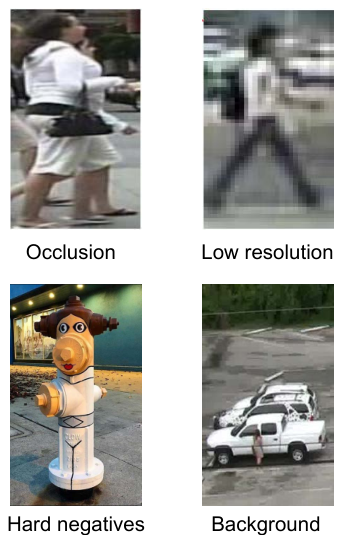
\includegraphics[height=10cm]{images/challenges.PNG}
    \caption{Challenges in trespassing detection system}
    \label{fig:challenges}
\end{figure}


\begin{comment}
\subsection{State of the art}
Person detection problem has been studied extensively by the computer vision community. While conventional techniques tend to develop hand-crafted features, more recent work (deep learning based approaches) attempt to learn features from the data. Most of the deep-learning based person detection work borrows ideas from the general object detection research and integrates some domain knowledge such as aspect ratio of up-right human and visible body parts. 

These works however do not intend to solve trespassing detection problem.
Most of the surveillance video is expected to be sparse in terms of trespassing activity. Thus direct application of existing methods leads to extra computational costs.
\end{comment}


\subsection{Proposed approach}
\label{sec:approach}
In order to fulfill our goals, we design a two step approach. Figure \ref{fig:trespassing-detection-framework} depicts the overall idea of our approach.  In the first step, we decide whether a particular frame has activity or not. If it turns out that the given frame has no activity, then it is classified as background frame. No further action needs to be taken for this frame. On the other hand, if it shows activity, then the next step will be to investigate whether it can be classified as human trespassing activity or not.

\begin{figure}
    \centering
    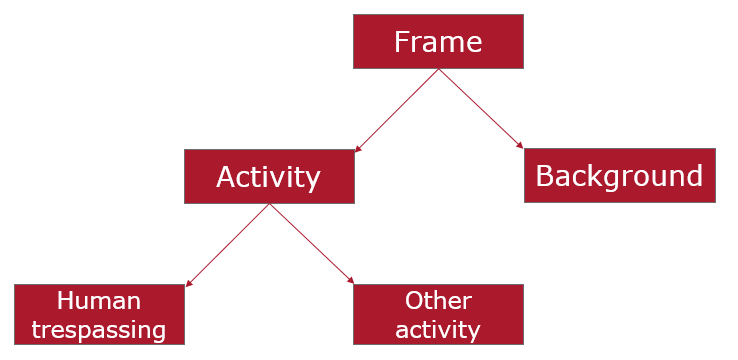
\includegraphics[width=\linewidth]{images/trespassing-detection-framework.PNG}
    \caption{Our approach}
    \label{fig:trespassing-detection-framework}
\end{figure}

% \subsection{Contribution}
% \subsection{Outline}


\newpage